\documentclass{standalone}
\usepackage{tikz}
\usetikzlibrary{shapes, arrows, positioning}

\begin{document}

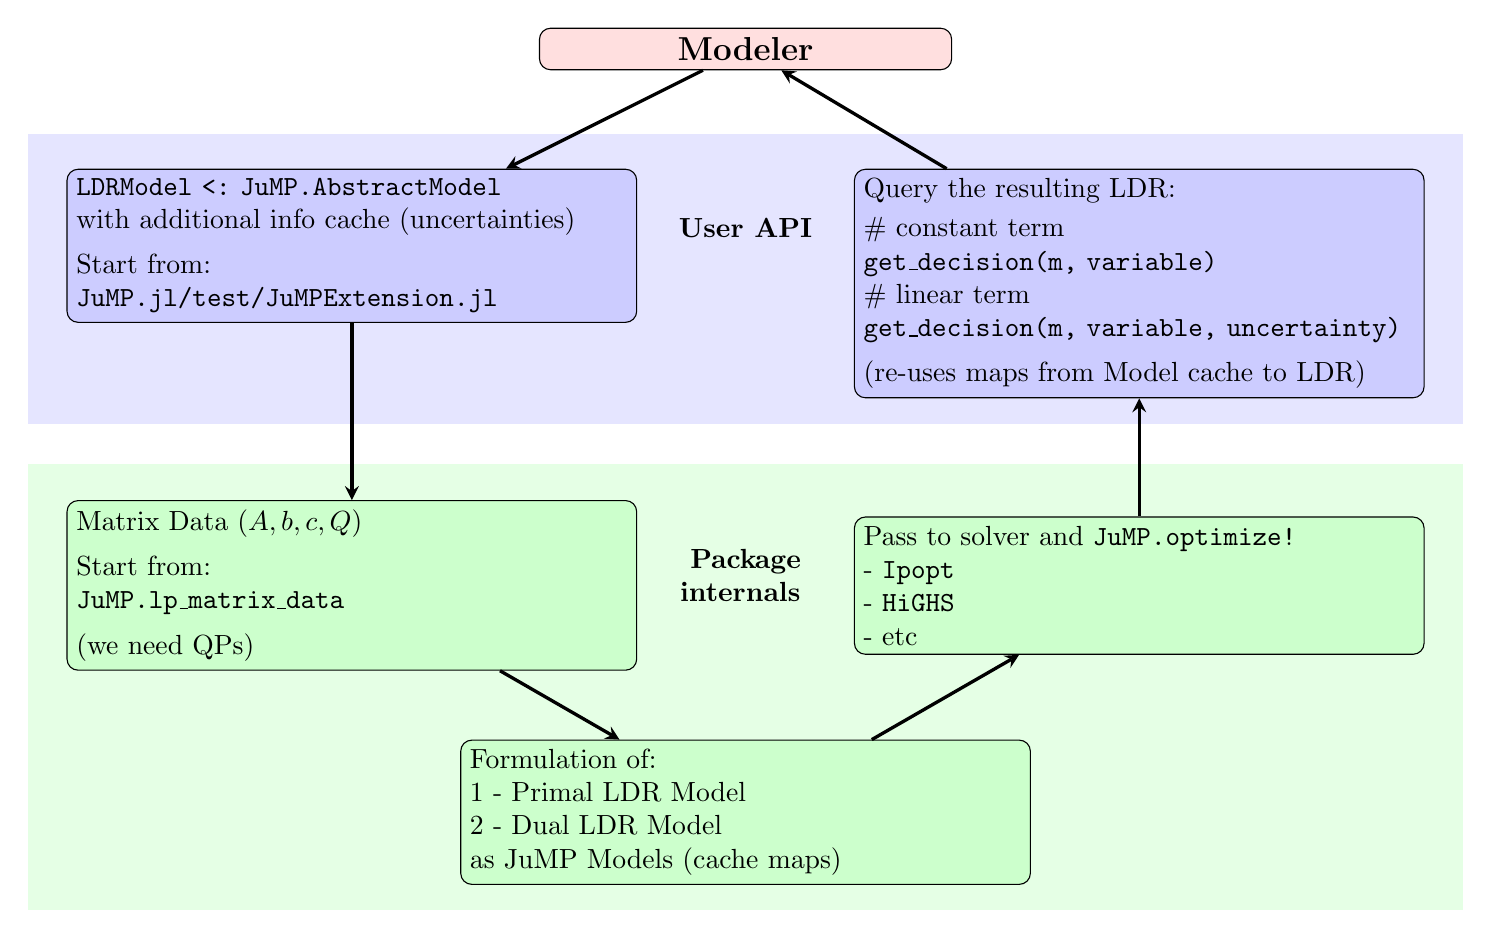
\begin{tikzpicture}[
    node distance=1.5cm and 1.5cm,
    box/.style={rectangle, draw, rounded corners, text width=7cm, align=left, fill=blue!20},
    header/.style={rectangle, draw, rounded corners, text width=5cm, align=center,
    fill=pink!50, font=\large\bfseries},
    process/.style={rectangle, draw, rounded corners, text width=7cm, align=left, fill=green!20},
    info/.style={font=\bfseries, text width=18cm, align=center},
    arrow/.style={very thick, ->, >=stealth}
]

% Nodes
\node[header] (modeler) {Modeler};

\node[info, below=of modeler, yshift=.7cm, text height=1.2cm, fill=blue!10]%
    (api) {User API\vspace{2.25cm}};
\node[box, below=of modeler, xshift=-5cm, yshift=.25cm] (userapi) {%
  \texttt{LDRModel <:\ JuMP.AbstractModel} \\
  with additional info cache (uncertainties) \\[1ex]
  Start from: \\
  \texttt{JuMP.jl/test/JuMPExtension.jl}
};
\node[box, below=of modeler, xshift=5cm, yshift=.25cm] (query) {%
  Query the resulting LDR: \\[.5ex]
    \# constant term \\
    \texttt{get\_decision(m, variable)} \\
    \# linear term \\
    \texttt{get\_decision(m, variable, uncertainty)} \\[1ex]
    (re-uses maps from Model cache to LDR)
};

\node[info, below=of api, yshift=1cm, fill=green!10, text height=1.2cm]%
  (package) {Package\\ internals \vspace{3.8cm}};
\node[process, below=of userapi, yshift=-.75cm] (matrixdata) {%
  Matrix Data $(A, b, c, Q)$ \\[1ex]
    Start from: \\
    \texttt{JuMP.lp\_matrix\_data} \\[1ex]
    (we need QPs)
};
\node[process, below=of modeler, yshift=-7cm] (formulation) {%
    Formulation of: \\
    1 - Primal LDR Model \\
    2 - Dual LDR Model \\
    as JuMP Models (cache maps)
};
\node[process, below=of query] (solver) {%
    Pass to solver and \texttt{JuMP.optimize!} \\
    - \texttt{Ipopt} \\
    - \texttt{HiGHS} \\
    - etc
};

% Arrows
\draw[arrow] (modeler) -- (userapi);
\draw[arrow] (userapi) -- (matrixdata);
\draw[arrow] (matrixdata) -- (formulation);
\draw[arrow] (formulation) -- (solver);
\draw[arrow] (solver) -- (query) ;
\draw[arrow] (query) -- (modeler);

\end{tikzpicture}

\end{document}

